\section*{Academic Integrity}
This statement is intended to cover most, but not all, forms of academic dishonesty. Please refer to The Rensselaer Handbook of Student Rights and Responsibilities for detailed information on Institute policy in this regard.

\textbf{Generative AI and AI-Assisted Technologies.} Regarding the use of Generative AI and AI-assisted technologies by students, the course policy is as follows:
\begin{itemize}
\item Only use these technologies to improve readability and language, not to replace key student learning tasks such as interpreting data or drawing analysis conclusions. Apply the technology with human oversight and control, and carefully review and edit the result, as AI can generate authoritative-sounding output that can be incorrect, incomplete, or biased.
\item Disclose in submissions the use of AI and AI-assisted technologies in the working process. Students are ultimately responsible and accountable for the contents of their submissions and must therefore be able to demonstrate that material generated has been cross-checked and verified from a different source/reference.
\end{itemize}

\textbf{Homework and Labs.} Collaboration among students in the class is permitted and encouraged. Seeking help from other sources is also encouraged. However, the work you submit should be your own. Students found to have copied any part of their homework from a solution manual or from an online database will be considered in breach of academic honesty. Appropriate recourse will sort based on the circumstances.

\textbf{Exams.} Collaboration during an exam (exchanging verbal or written information or copying) is prohibited. In addition, use of email or the internet during exams for any purpose is prohibited. All mobile devices (smart phones, computers, etc.) must be stored securely away during exams and are not to be used unless specifically directed otherwise by the instructor. Use of (or ANY interaction with) a mobile device during an exam without explicit permission of the instructor will be interpreted as the illicit transfer of exam data, will be considered an act of cheating, and will be treated as such. All parties involved will receive an F in the course.

\section*{Semester Timeline}
\vspace{0.25em}
\noindent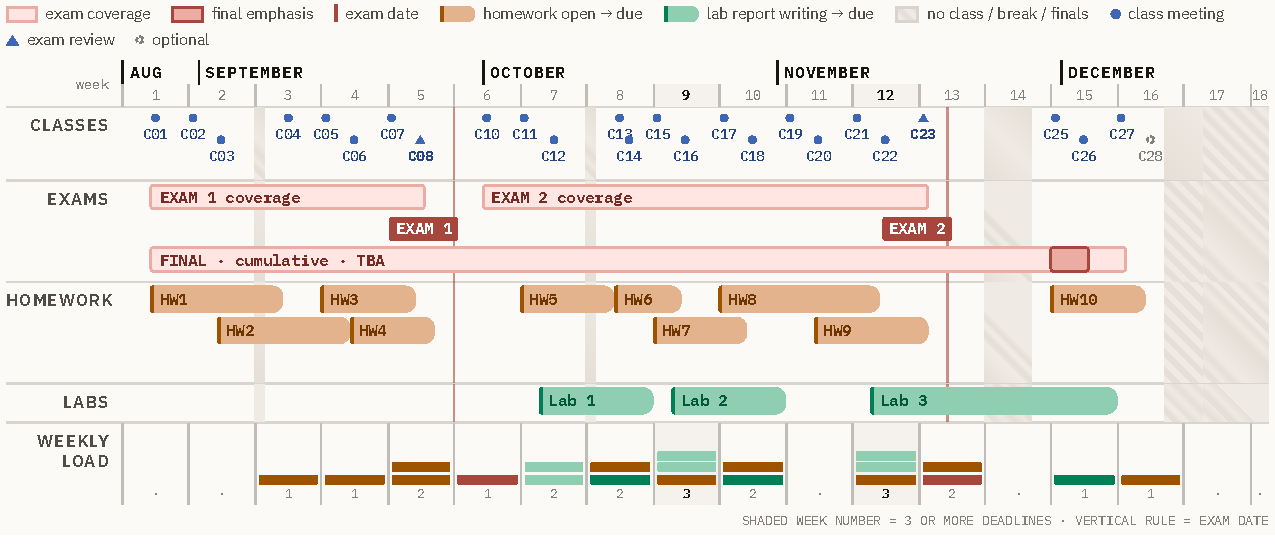
\includegraphics[width=\textwidth]{generated/visual_schedule_strip.pdf}

